\section{Problemanalyse und Realisation}
\subsection{Problemanalyse}
Hierbei habe ich mich einer Technik bedient in der man versucht sich in eine jeweilige Teilkomponente des Problems hineinzuversetzen und anzugeben fuer welchen Teilbereich diese Komponente verantwortlich ist. Anschliessend ist es etwas einfach sowie uebersichtlicher sich auf die Struktur festzulegen, da man s"amtliche Nomen als Klassen ansehen kann (hier einmal \colorbox{Apricot}{orange} dargestellt). Verben spiegeln die benoetigten Methoden wieder (hier \colorbox{SpringGreen}{gruen} dargestellt).

\begin{enumerate}
	\item Benutzer
	\begin{enumerate}
		\item als \colorbox{Apricot}{Benutzer} möchte ich den aktuellen Spielstand in eine Datei mit Auswahl des Dateinamens \colorbox{SpringGreen}{speichern}. Das Logging wird mit \colorbox{SpringGreen}{gespeichert}.
		\item als \colorbox{Apricot}{Benutzer} möchte ich eine Datei mit einem Spielstand  \colorbox{SpringGreen}{auswählen} und \colorbox{SpringGreen}{öffnen} können.
		\item als \colorbox{Apricot}{Benutzer} möchte ich ein \colorbox{Apricot}{Spiel} initialisieren und neu starten.
		\item als \colorbox{Apricot}{Benutzer} möchte ich ein \colorbox{Apricot}{Spiel} \colorbox{SpringGreen}{beenden}mit/ohne zu \colorbox{SpringGreen}{speichern}.
		\item als \colorbox{Apricot}{Benutzer} möchte ich das Laden oder Speichern  \colorbox{SpringGreen}{loggen}.
	\end{enumerate}	
	\item Spieler
	\begin{enumerate}
		\item als \colorbox{Apricot}{Spieler} möchte ich einen \colorbox{Apricot}{Domino} \colorbox{SpringGreen}{auswählen}.
 		\item als \colorbox{Apricot}{Spieler} möchte ich einen \colorbox{Apricot}{Domino} \colorbox{SpringGreen}{drehen}.
		\item als \colorbox{Apricot}{Spieler} möchte ich einen \colorbox{Apricot}{Domino} \colorbox{SpringGreen}{setzen}.
		\item als \colorbox{Apricot}{Spieler} möchte ich das Stadtzentrum \colorbox{SpringGreen}{bewegen}.
		\item als \colorbox{Apricot}{Spieler} möchte ich meine Aktionen \colorbox{SpringGreen}{loggen}.
	\end{enumerate}
	\item Spiel
	\begin{enumerate}
		\item als \colorbox{Apricot}{Spiel} möchte ich die \colorbox{Apricot}{Spielfelder} der Spieler \colorbox{SpringGreen}{visualisieren}.
		\item als \colorbox{Apricot}{Spiel} möchte ich die \colorbox{Apricot}{Auswahlfelder} \colorbox{SpringGreen}{visualisieren}.
		\item als \colorbox{Apricot}{Spiel} möchte ich den aktuellen Spielstand der Spieler \colorbox{SpringGreen}{anzeigen}.
		\item als \colorbox{Apricot}{Spiel} möchte ich den \colorbox{Apricot}{Gewinner} \colorbox{SpringGreen}{anzeigen}
		\item als \colorbox{Apricot}{Spiel} möchte ich den \colorbox{Apricot}{Gewinner} \colorbox{SpringGreen}{loggen}.
	\end{enumerate}
\end{enumerate}

\subsection{Realisationsanalyse}
\paragraph{Grunds"atzlich ben"otigte Datenstrukturen}
Um eine Partie spielen zu k"onnen werden erst einmal Spielsteine ben"otigt. Hierbei wurden diverse Klassen eingef"uhrt die im Kapitel \nameref{par:domino} \ref{par:domino} auf Seite \pageref{par:domino}
genauer beschrieben werden. Letztendich bieten diese allerdings s"aemtliche ben"otigte Schnittstellen um einen Domino mit einer bestimmten Aufschrift an mit einer Position zu versehen. 

Diese Dominos k"onnen auf Spielbrettern positioniert werden. Jeder Spieler besitzt hierbei eins, und die Gui ist in der Lage diese ordnungsgem"ass darzustellen. 

Um einen Domino w"ahlen zu k"onnen ist es essentiell ein Konstrukt f"ur eine Bank zu implementieren. Ich habe dabei eine eine Struktur gew"ahlt in der s"amtliche Spieler nicht anhand irgendeines Indices, sondern anhand ihrer Referenz gespeichert werden. Dies erm"oglicht eine genaue Zuordnung, da es ja m"oglicherweise Spieler mit identischem Index geben k"onnte. 

\paragraph{Benutzerschnittstelle}
Der Punkt Benutzer entspricht in diesem Projekt s"amtlichen Anfragen die ein Benutzer dem Programm stellen kann. Es bietet sich an eine Struktur zu waehlen in der eine Klasse oder Schnittstelle als Anlaufstelle dient ueber die sämtliche Anfragen bearbeitet werden koennen. Hierbei ist nur abzuwaegen ob man eventuell die \glqq Antwort\grqq  des Programms gleich in diese Schnittstelle mit aufnimmt. Dies führt allerdings zu unuebersichtlichem Code. 

\paragraph{Spielerverhalten}
Der Punkt Spieler beschreibt die wirklichen Spielteilnehmer. Er muss in der Lage sein selbststaendig oder durch die Interatktion mit der Gui einen Zug vollziehen zu koennen. Hierzu gehoert das auswahlen, drehen und setzen eines Dominos. Hier gilt es abzuwaehlen ob dies durch eine gemeinsame Klasse geschehen soll, ich habe mich allerdings fuer eine Unterteilung entschieden da der menschliche Spieler auf die Eingabe des Benutzers, ueber die Benutzerobflaeche, abarbeitet, waehrend die Bots diese mehr oder weniger ignorieren und isoliert ihre Zuege vollziehen. 

Desweiteren ben"otigt der Spieler ein Spielbrett auf dem er Dominos setzen kann. Man k"onnte das Spielbrett auch der Verwaltung (also der Spiel-Klasse) "uberlassen, dann w"aere ein Spieler aber nicht mehr so unabh"angig vom Spiel wie in diesem Fall. Es ist so m"oglich eine minimale Schnittstelle dem Spiel gegen"uber bereitzustellen, indem der Spieler selbst alle wichtigen Schritte ausf"uhrt um einen Zug zu machen. 

Die Kapsellung des Spielerverhaltens erm"oglicht es ausserdem wartbaren Code zu erzeugen. Es ist einfacher Fehler zu beheben oder bestimmte Prozesse auszutauschen ohne das komplette Programm umstrukturieren zu m"ussen, aber am wichtigsten hierbei ist die M"oglichkeit der Erweiterbarkeit. Durch die Kapselung ist es m"oglich s"amtliche Schritte eines Spielers polymorph zu gestalten. Jede Spielerart reagiert also anders auf eine Anfrage und es nicht n"otig den Aufruf hierf"ur zu ver"andern. All diese M"oglichkeiten w"urden entfallen, wenn man das Spielverhalten der k"unstlichen Spieler in der Spiel-Klasse aufrufen w"urde.

\paragraph{Spielerinstantiierung}
Um die Bindung zum Spiel so gering wie m"oglich zu halten (wie im letzten Absatz erkl"art). Habe ich versucht auch bei der Instantiierung m"oglichst nachhaltigen Code zu schreiben indem ich eine statische Fabrikmethode verwende um die einzelnen Spieler zu instantiieren. Letztendlich verschiebt man mit solch einer einfach Fabrik lediglich die Instantierung in eine gemeinsame Methode, allerdings muss man im sp"ateren Verlauf der Entwicklung auch nur hier Dinge "andern. Dies ist besonders hilfreich beim hinzuf"ugen weiterer Spielertypen. Die Fabrik-Methode befindet sich in einem Enum namens \emph{Playertypes}. Diese Enum-Werte k"onnen in gewisser Weise aber auch als Platzhalter f"ur die \glqq richtigen\grqq  Spieler herhalten. Wie das funktioniert wird im folgendem Abschnitt beschrieben. 

\paragraph{Alternative Spielerinitialisierung}
\label{par:alternativeSpielerinitialisierung}
Der Vorgang des Instantiierens in der Fabrik-Methode ist relativ aufwendig. Man h"atte s"amtliche Operationen theoretisch auch im Konstruktor behandeln k"onnen, auf lange Sicht ist es aber effektiver Sie hier anzusiedeln da man sonst nur sehr umst"andlich ein Auswahlfeld f"ur m"ogliche Spieler starten kann. Hierzu folgendes Szenario: Es gibt N Spielertypen unter denen der Benutzer seine Gegner w"ahlen kann. Daf"ur gibt es ein eigenes Auswahlfenster, welches vor dem eigentlichen Spiel auftauchen soll (siehe Abbildung \ref{fig:auswahlfenster}, S. \pageref{fig:auswahlfenster}). Der Controller dieses Fensters "ubernimmt somit die Aufgabe der Main-Methode das Spiel zu starten. Diese tut genau dasselbe wie die urspr"ungliche Main-Methode indem Sie das FXML-Dokument aufruft. Der Controller wird dabei automatisch gestartet und die Initialize-Methode der Controller-Klasse des GameFXML-Dokuments durchlaufen. Hierbei habe ich bei meinen "Uberlegungen keinen Weg gefunden Argumente der Initialize-Methode zu "ubergeben, da diese ja das Interface Initializable implementiert und somit die Signatur nicht ver"andert werden kann. Daher gibt es eine eine Methode welche losgel"ost vom Konstruktor das Spiel mit "ubergebenen Spielertypen starten kann. Dieser Ansatz funktioniert soweit und ist in der Main-Klasse als auskommentierter Block mit dem Schl"usselwort \glqq Alternative\grqq  gekennzeichnet. Falls dieser Block einkommentiert und der Rest der Main-Methode auskommentiert wird startet ein Auswahlfenster mit einer M"oglichkeiten der Spielerselektierung. Dies ist allerdings noch nicht ausgereift da es lediglich zur Darstellung des Problems dienen soll, sodass bei invalider Selektierung eine Exception geworfen wird.

\begin{figure}
	\centering
	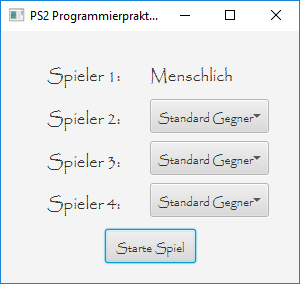
\includegraphics[width=.4\linewidth]{pics/Intro240918}
	\caption[Auswahlfenster]{Auswahlfenster}
	\label{fig:auswahlfenster}
\end{figure}

\paragraph{Spiel}
Dieser Begriff beschreibt koordinierte Abarbeitung der Spielerzuege. Es wird der Benutzeroberflaeche mitgeteilt was angezeigt werden soll. Ausserdem werden saemtliche saemtliche Stapel von Dominos bereitgestellt die fuer ein vollwertiges Spiel genutzt werden sollen (Beutel, Baenke). Alle benoetigten Dateioperationen werden hier eingeleitet aber nicht direkt in dieser Klasse bearbeitet. Durch das ganze Exceptionhandling wird es ziemlich unuebersichtlich alles in das Spiel zu packen, da dieses in erster Linie fuer die uebergeordnete Organisation des ganzen Programms gedacht ist. 

\paragraph{Log}
Da man vermehrt, und vor allem an vielen verschiedenen Stellen im Code, eine neue Zeile in die Logdatei schreiben beziehungsweise auf der Konsole ausgeben m"ochte, bietet sich f"ur die Implementierung des Loggers das \emph{singleton Muster} an. Dieses Muster verwaltet eine einzige globale Instanz auf die immer wieder drauf zugegriffen wird. Das Muster wird eignet sich besonders gut fuer das Loggen von Daten, da man alles in die selbe Datei schreiben m"ochte und diese nicht jedesmal neu \emph{suchen} muss. Im Logger kann man zum Beispiel einfach ein entsprechendes Feld anlegen. 

\paragraph{Speichern und Laden}
Auch beim Speichern und Laden wird in diesem Entwurf ein \emph{singleton Muster} verwendet. Da man beim Speichern jeweils den Dateipfad nach erstmaliger Eingabe nicht erneut eingeben m"ochte wenn dies nicht unbedingt erforderlich ist (siehe Abschnitt 
\emph{Speichern als} gegen"ueber \emph{Speichern}, \ref{spar:anleitung_speichern} auf Seite \pageref{spar:anleitung_speichern}). Und auch das Speichern und Laden tritt immer wieder vermehrt und verteilt ueber den gesamten Code auf. Alternativ k"onnte man auch ein klassische Klasse verwenden, wegen den genannten Punkten empfiehlt sich aber gerade f"ur diese beiden Anwendungsf"alle dieses Muster. F"ur eine genauere Beschreibung des Musters siehe \ref{par:singletonMuster} \nameref{par:singletonMuster} auf Seite \pageref{par:singletonMuster}. 
